\documentclass[compress, darktitle, framenumber, totalframenumber]{beamer}
\usepackage{booktabs}
\usepackage{mathtools}
\usepackage{siunitx}
\usepackage{tikz}
\usepackage{wasysym}
\usepackage{wrapfig}
\usepackage{xparse}

\mathtoolsset{showonlyrefs}

\newcommand\frequencydiagram[5]{
  % TODO change number of samples
  \begin{tikzpicture}[scale = 0.85, domain = 0:10, samples = 500]
    \draw[very thin] (-0.1,-2.1) grid (10.1,2.1);
    \draw[thick, ->] (-0.2,0) -- (10.2,0);

    \draw[fill] (0,0) circle (2pt) node [below left] {$0$};
    \draw[fill] (pi,0) circle (2pt) node [below] {$\pi$};
    \draw[fill] (2*pi,0) circle (2pt) node [below] {$2\pi$};
    \draw[fill] (3*pi,0) circle (2pt) node [below] {$3\pi$};

    \draw[color = vividbrown] plot function{sin(#1*#2*x)} node[right] {\SI{#4}{\hertz}};
    \draw[color = uared] plot function{sin(#1*#3*x)} node[right] {\SI{#5}{\hertz}};

    \pause
    \draw[color = vividbrown!40] plot function{sin(#1*#2*x)} node[right] {\SI{#4}{\hertz}};
    \draw[color = uared!40] plot function{sin(#1*#3*x)} node[right] {\SI{#5}{\hertz}};
    \draw[semithick, color = uablue] plot function{2*sin(#1*(#3+#2)*x/2)*cos(#1*(#3-#2)*x/2)} node[right] {som};
  \end{tikzpicture}
}

\usetheme{UniversiteitAntwerpen}
\beamertemplatenavigationsymbolsempty

\title{Wisku$\mathbb{N}$de in-$\mathbb{Z}$icht}
\subtitle{Wiskunde in muziek}
\author{Pieter Belmans (\texttt{pieter.belmans@uantwerpen.be}) \\ Matthias Roels (\texttt{matthias.roels@uantwerpen.be})}
\date{9 januari 2014}

\begin{document}
\begin{frame}
  \titlepage
\end{frame}

\begin{frame}
  \frametitle{Wie zijn wij?}
\end{frame}

\begin{frame}
  \frametitle{Wat gaan we vandaag doen?}

  \begin{block}{Voormiddag}
    \begin{wrapfigure}{r}{.5\textwidth}
      \centering
      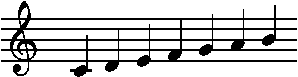
\includegraphics{scores/scale-cropped}
    \end{wrapfigure}
    Waarom do-re-mi-fa-sol-la-si?
    \begin{enumerate}
      \item de structuur van geluid
      \item mooi en lelijk
      \item 7 (of 12) noten
    \end{enumerate}
  \end{block}

  \pause

  \begin{block}{Namiddag}
    Wat maakt geluid muziek?
    \begin{enumerate}
      \item de structuur van geluid analyseren
      \item voorbeelden
      \item verschillen tussen muziekinstrumenten
    \end{enumerate}
  \end{block}
\end{frame}

\begin{frame}
  \frametitle{Vragen staat vrij}

  Voorkennis (?):
  \begin{enumerate}
    \item de sinus
    \item goniometrische formules
    \item rekenen met logaritmes
    \item muziek: noten lezen, enige terminologie
  \end{enumerate}
\end{frame}

\section{Wat is geluid?}

\section{Wat zijn boventonen?}
% TODO refer to last part of talk, and afternoon

\begin{frame}
  \frametitle{Staande golven}

  We experimenteren met touw
\end{frame}

\begin{frame}
  \frametitle{Boventonen}

  \centering
  \begin{tikzpicture}[scale = .7]
    \foreach \k in {1,...,7} {
      \draw[smooth, domain = 0:3*pi, samples = 100] plot (\x,{sin(60*\k*\x/pi)/5-\k});
      \draw[smooth, domain = 0:3*pi, samples = 100] plot (\x,{-sin(60*\k*\x/pi)/5-\k});
      \draw[fill] (0,-\k) circle (1pt);
      \draw[fill] (3*pi,-\k) circle (1pt);
    };

    \draw (3*pi,-1) node[above, uablue, font = \tiny] {$1$};
    \foreach \k in {2,...,7} {
      \draw[fill, uablue!60] (3*pi/\k,-\k) circle (1pt) node[above, uablue, font = \tiny] {$1/\k$};
    };
  \end{tikzpicture}
\end{frame}

\section{Wat klinkt er mooi samen en wat niet?}

\begin{frame}
  \frametitle{We luisteren naar boventonen}

  De boventonen hebben een sterk verband met de grondtoon, en geven een mooie samenklank.

  \pause

  Als sinussen:
  \begin{block}{\twonotes\ audiofragmenten}
    \texttt{samples/440-880.mp3} \\
    \texttt{samples/440-880-878.mp3} \\
  \end{block}

  \pause
  Conclusie:
  \begin{enumerate}
    \item gehele veelvouden klinken mooi samen
    \item n\'et niet gehele veelvouden klinken lelijk
  \end{enumerate}
\end{frame}

\begin{frame}
  \frametitle{Nu met echte instrumenten}

  \begin{block}{\twonotes\ audiofragmenten}
    %TODO we need more samples here! preferably with real instruments!
  \end{block}

  \pause

  \begin{alertblock}{Conclusie}
    Ons gehoor houdt van gehele veelvouden.
  \end{alertblock}
\end{frame}

\begin{frame}
  \frametitle{Het samen laten klinken van twee geluidsgolven}

  Wat gebeurt er als we twee frequenties~$f_1$ en~$f_2$ laten horen?
  \begin{equation}
    \sin(f_1t)+\sin(f_2t)=\onslide<1>{?}\pause\!\!\!2\sin\left( \frac{f_1+f_2}{2}t \right)\cos\left( \frac{f_1-f_2}{2}t \right).
  \end{equation}

  \pause

  Welke conclusies zijn er te trekken?

  \pause

  \begin{enumerate}
    \item de factor 2 levert ons dat het signaal tot dubbel zo sterk kan worden;
    \item de sinus of cosinus in het product kan 0 zijn.
  \end{enumerate}

\end{frame}

\begin{frame}
  \frametitle{Voorbeeld}

  Stel $f_1=\SI{2}{\hertz}$ en $f_2=\SI{3}{\hertz}$:

  \begin{center}
    \frequencydiagram{2}{1}{1.5}{2}{3}
  \end{center}

  \onslide<2>{Soms versterken de twee signalen elkaar, soms verzwakken ze elkaar.}
\end{frame}

\begin{frame}
  \frametitle{Voorbeeld}

  Stel $f_1=\SI{3}{\hertz}$ en $f_2=\SI{4}{\hertz}$:

  \begin{center}
    \frequencydiagram{3}{1}{1.3333}{3}{4}
  \end{center}

  \onslide<2>{Het versterken en verzwakken is (uiteraard) ook periodisch.}
\end{frame}

\begin{frame}
  \frametitle{Voorbeeld}

  Stel $f_1=\SI{3}{\hertz}$ en $f_2=\SI{5}{\hertz}$:

  \begin{center}
    \frequencydiagram{3}{1}{1.666}{3}{5}
  \end{center}

  \onslide<2>{Golven kunnen \alert{in fase} of \alert{uit fase} zijn.}
\end{frame}

\begin{frame}
  \frametitle{Zweving}

  Wat als~$f_1$ en~$f_2$ bijna hetzelfde zijn?
  
  Stel $f_1=\SI{8}{\hertz}$, $f_2=\SI{9}{\hertz}$:

  \begin{center}
    \frequencydiagram{8}{1}{1.125}{8}{9}
  \end{center}
\end{frame}

\begin{frame}
  \frametitle{Nog meer zweving}

  Stel $f_1=\SI{16}{\hertz}$, $f_2=\SI{17}{\hertz}$:

  \centering
  \frequencydiagram{16}{1}{1.0625}{16}{17}

  \onslide<2>{We zien opnieuw een golfpatroon met frequentie $\SI{1}{\hertz}=\SI{17}{\hertz}-\SI{16}{\hertz}$}
\end{frame}

\begin{frame}
  \frametitle{Zweving}

  Hoe klinkt dit nu?

  \begin{block}{\twonotes\ audiofragment}
    %TODO we need more samples here!
  \end{block}
\end{frame}

\begin{frame}
  \frametitle{Zweving}

  \begin{block}{\twonotes\ audiofragmenten}
    \texttt{samples/440-880-878.mp3} \\
    % TODO some other real sound sample showing beating
  \end{block}

  \pause

  \begin{alertblock}{Definitie}
    Het luider en stiller worden van het geluid noemen we \emph{zweving} (of \emph{beating} in het Engels).
  \end{alertblock}

  \begin{enumerate}
    \item instrumenten die niet goed gestemd zijn geven zulke zwevingen
    \item zweving kan best vermeden worden (maar soms is het intentioneel, zeker in moderne muziek)
  \end{enumerate}
\end{frame}

\section{Hoe maken we verschillende noten?}

\begin{frame}
  \frametitle{Gehele veelvouden}

  Muziek met 1 noot zou maar saai zijn. Hoe kiezen we de andere noten? \pause We willen
  \begin{enumerate}
    \item mooie samenklank
    \item \pause genoeg noten om interessante muziek te schrijven
    \item \pause niet te veel noten om de muziek nog speelbaar te houden
  \end{enumerate}

  We hebben een goede leidraad voor mogelijke nieuwe noten: de \alert{boventonen}! De eerste voorwaarde is alvast voldaan.

  Hoe gaan we verder?
\end{frame}

\begin{frame}
  \frametitle{De kwint}

  De \alert{eerste boventoon} ``klinkt hetzelfde'', de verdubbeling in frequentie levert geen echt verschil op, we noemen dit een \alert{octaaf}.

  \pause

  Om hem te spelen op een snaar moeten we de snaarlengte \emph{halveren}.

  \pause
  \vspace{1em}

  De \alert{tweede boventoon} (dus 3 maal de grondfrequentie) klinkt w\'el anders!

  \begin{enumerate}
    \item De snaar \emph{in drie delen} levert deze frequentie als grondtoon.
    \item \pause De snaar dan weer in lengte verdubbelen levert een mooie toon die niet te ver van de grondtoon ligt: hij is dus $3/2$ keer de grondfrequentie.
  \end{enumerate}
  Het resultaat noemen we een \alert{kwint}.
\end{frame}

\begin{frame}
  \frametitle{Octaven en kwinten}

  We horen nu de grondtonen met frequenties $\SI{220}{\hertz}$ (= la) en $\SI{330}{\hertz}$ (= mi)
  \begin{block}{\twonotes\ audiofragmenten}
    \begin{wrapfigure}{r}{.4\textwidth}
      \vspace{-.5cm} % weird hack to get position right
      \centering
      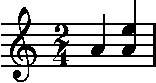
\includegraphics{scores/fifths-cropped}
    \end{wrapfigure}

    % TODO these should be made with a real piano sound!
    \texttt{samples/octave.mp3} \\
    \texttt{samples/fifth.mp3} \\
    \texttt{samples/octave-fifth.mp3}
  \end{block}
\end{frame}

\begin{frame}
  \frametitle{Kwinten visueel}

  \begin{center}
    \frequencydiagram{22}{1}{1.5}{22}{33}
  \end{center}
\end{frame}

\begin{frame}
  \frametitle{Kwinten visueel}

  Wat als we net geen verhouding van $3/2$ hebben?
  \begin{center}
    \frequencydiagram{22}{1}{1.5454}{22}{34}
  \end{center}
\end{frame}

\begin{frame}
  \frametitle{De terts}

  De \alert{vierde boventoon} is een verviervoudiging van de grondfrequentie, dus \alert{twee octaven}.

  \pause
  \vspace{1em}

  De \alert{vijfde boventoon} is w\'el nieuw. We hebben $5/4$ keer de grondfrequentie.
\end{frame}

\begin{frame}
  \frametitle{Octaven, kwinten en tertsen}

  We horen nu de grondtonen met frequenties $\SI{220}{\hertz}$ (= la), $\SI{275}{\hertz}$ (= do\#) en $\SI{330}{\hertz}$ (= mi)
  \begin{block}{\twonotes\ audiofragmenten}
    \begin{wrapfigure}{r}{.4\textwidth}
      \vspace{-.5cm} % weird hack to get position right
      \centering
      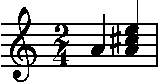
\includegraphics{scores/major-chord-cropped}
    \end{wrapfigure}

    \texttt{samples/thirds.mp3} \\
    \texttt{samples/fifths-thirds.mp3} \\
    \texttt{samples/major-chord.mp3}
  \end{block}

  \pause

  We misbruiken hier natuurlijk de notatie die we pas kunnen invoeren als we het systeem volledig bedacht hebben.
\end{frame}

\begin{frame}
  \frametitle{Een toonladder bouwen}

  We hebben nu de basis voor onze muziek in handen:
  \begin{enumerate}
    \item kwinten;
    \item tertsen.
  \end{enumerate}
  We kunnen deze stapelen, om zo nieuwe noten te vormen.
\end{frame}

\begin{frame}
  \frametitle{Pythagoras}

  % music of the spheres etc
\end{frame}

\section{Wat is een stemming?}
% TODO: answers the question ``why do we have C D E F G A B''
% from here on: leave the world of Pythagoras and get your hands dirty on getting it right

\section{Wat is het probleem met stemmingen?}

\begin{frame}
  \frametitle{Dezelfde noot, of toch niet?}

  neem een grondnoot (bijvoorbeeld de do), en beschouw
  \begin{enumerate}
    \item 7 octaven erboven: opnieuw een do
      \pause
    \item 12 kwinten erboven: \\
      do sol re la mi si fa\# do\# sol\# re\# la\# mi\# si\#

      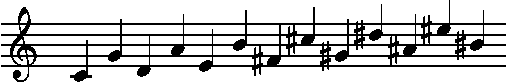
\includegraphics{scores/circle-cropped}
  \end{enumerate}
  \pause
  in frequenties:
  \begin{description}
    \item[grondnoot:] $\SI{100}{\hertz}$ (om de getallen mooier te maken!)
    \item[7 octaven:] $2^7\cdot\SI{100}{\hertz}=\SI{12800}{\hertz}$ 
      \pause
    \item[12 kwinten:] $(3/2)^{12}\cdot\SI{100}{\hertz}\approx\SI{12975}{\hertz}$
  \end{description}
\end{frame}

\begin{frame}
  \frametitle{Dezelfde noot: si\# = do}

  We brengen alles 7 octaven naar beneden:
  \begin{description}
    \item[grondnoot:] $\SI{100}{\hertz}$
    \item[12 kwinten:] $(3/2)^{12}/2^7\cdot\SI{100}{\hertz}\approx\SI{101.36}{\hertz}$
  \end{description}
  \pause
  \begin{block}{\twonotes\ audiofragment}
    \texttt{samples/7-12-glissando-400Hz.mp3} \\
    \texttt{samples/7-12-400Hz.mp3}
  \end{block}
  \pause
  We willen si\# = do zodat we slechts 12 noten moeten gebruiken in onze muziek.

  \begin{alertblock}{Vraag}
    Is dit de enige mogelijke keuze?
  \end{alertblock}
\end{frame}

\begin{frame}
  \frametitle{Waarom het nooit kan kloppen}

  \begin{block}{Antwoord}
    Dit is niet de enige mogelijke keuze!
  \end{block}
  We bouwen onze toonladder op met behulp van octaven en kwinten. En we willen op een bepaald moment twee noten gelijkstellen.

  \pause
  Dat betekent:
  \begin{equation}
    2^n=\left( \frac{3}{2} \right)^m
  \end{equation}
  voor~$m$ en~$n$ natuurlijke getallen. Op de vorige slide: $n=7,m=12$.
  \pause
  \begin{alertblock}{Vraag}
    Zijn er perfecte keuzes mogelijk?
  \end{alertblock}
\end{frame}

\begin{frame}
  \frametitle{Waarom het nooit kan kloppen}

  \begin{block}{Antwoord}
    Nee!
  \end{block}
  \pause
  \begin{equation}
    \begin{aligned}
      2^n=\left( \frac{3}{2} \right)^m&\Longleftrightarrow 2^{n+m}=3^m
    \end{aligned}
  \end{equation}
  maar het linkerlid is even, het rechterlid oneven.
\end{frame}

\section{Hoe kunnen we dit oplossen?}

\section{Hoe kan geluid ons bedotten?}
% TODO: end the previous section with a remark hinting at the crappy way we experience sound, ties it in with this last section *and* afternoon
\begin{frame}
  \frametitle{Illusies met geluid}

  % http://tex.stackexchange.com/questions/129274/showcase-of-optical-illusions-made-with-tex-latex-luatex-context
  \centering
  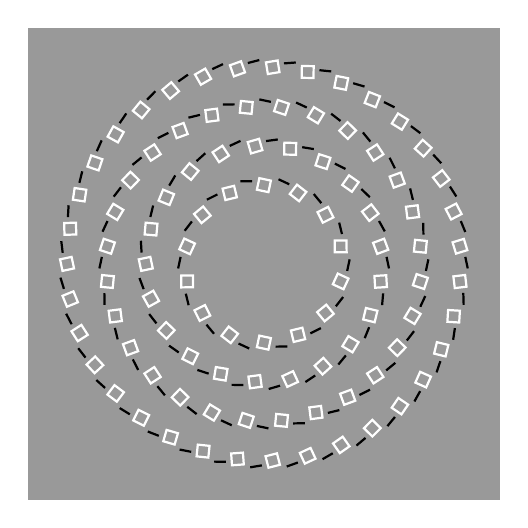
\begin{tikzpicture}[scale = .5]
    \fill[color=black!40!white] (-6,-6) rectangle (6,6);
    \foreach \n/\r/\twist in {70/5/12,56/4/-12,42/3/12,28/2/-12}{
      \foreach \m in {1,3,...,\n}
        \draw [thick,color=white,shift={(360/\n*\m:\r)},rotate=\twist+360/\n*\m] (-.15,-.15) rectangle (.15,.15);
      \foreach \m in {2,4,...,\n}
        \draw [thick,color=black,shift={(360/\n*\m:\r)},rotate=\twist+360/\n*\m] (.15,-.15) rectangle (.15,.15);
      }
  \end{tikzpicture}
\end{frame}

\begin{frame}
  \frametitle{Hoe do-re-mi-fa-sol-la-si ons bedot}

  We weten nu dat
  \begin{center}
    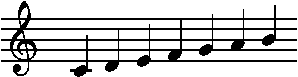
\includegraphics{scores/scale-cropped}
  \end{center}
  overeenkomt met
  \begin{center}
    \begin{tabular}[h]{cccccccc}
      do & re & mi & fa & sol & la & si \\\midrule
      131Hz & 147Hz & 165Hz & 175Hz & 196Hz & 220Hz & 247Hz
    \end{tabular}
  \end{center}
\end{frame}

\begin{frame}
  \frametitle{Een oneindig stijgende toonladder}

  Nu gebruiken we alle twaalf tonen:
  \begin{center}
    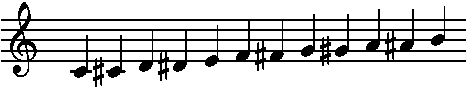
\includegraphics{scores/scale-full-cropped}
  \end{center}
  De frequenties zijn niet zo belangrijk\ldots
\end{frame}

\begin{frame}
  \frametitle{Een toonladder}

  \begin{block}{\twonotes\ audiofragment}
    \texttt{samples/endless.mp3}
  \end{block}
  \pause
  \begin{center}
    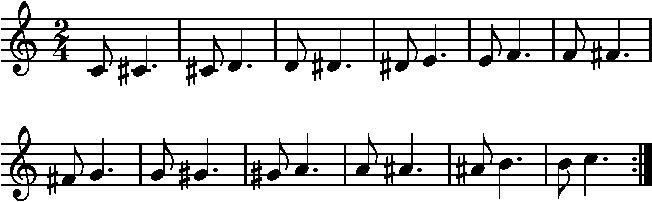
\includegraphics{scores/endless-cropped}
  \end{center}
  \pause
  De toonladder \alert{herhaalt} zich, zonder overgang!
\end{frame}

\begin{frame}
  \frametitle{Wat is er aan de hand?}

  We analyseren het geluid
  % TODO
\end{frame}

\begin{frame}
  \frametitle{Observaties}

  \begin{enumerate}
    \item (alles is een beetje te laag gestemd)
    \item er is geen vastomlijnde grondtoon
    \item de duidelijkste frequentie wordt \alert{zwakker}
    \item de nauwelijks aanwezige laagste frequentie wordt \alert{sterker}
    \item de laatste toon heeft dezelfde samenstelling als de eerste
  \end{enumerate}
\end{frame}

\begin{frame}
  \frametitle{Herhaalde geluidsanalyse}

  We analyseren meerdere kopies van het fragment
  % TODO
\end{frame}

\begin{frame}
  \frametitle{Observaties}

  \begin{enumerate}
    \item we horen de overgang niet, maar \alert{zien} hem wel
    \item exponenti\"eel stijgend
  \end{enumerate}
\end{frame}

\begin{frame}
  \frametitle{Paradox van Shepard}
\end{frame}

\begin{frame}
  \frametitle{Een oneindig dalende glissando}

  Een continue versie van voorgaande paradox
  \begin{block}{\twonotes\ audiofragment}
    \texttt{samples/shepard-risset-glissando.ogg}
  \end{block}
\end{frame}

\begin{frame}
  \frametitle{Paradox van Shepard--Risset}

  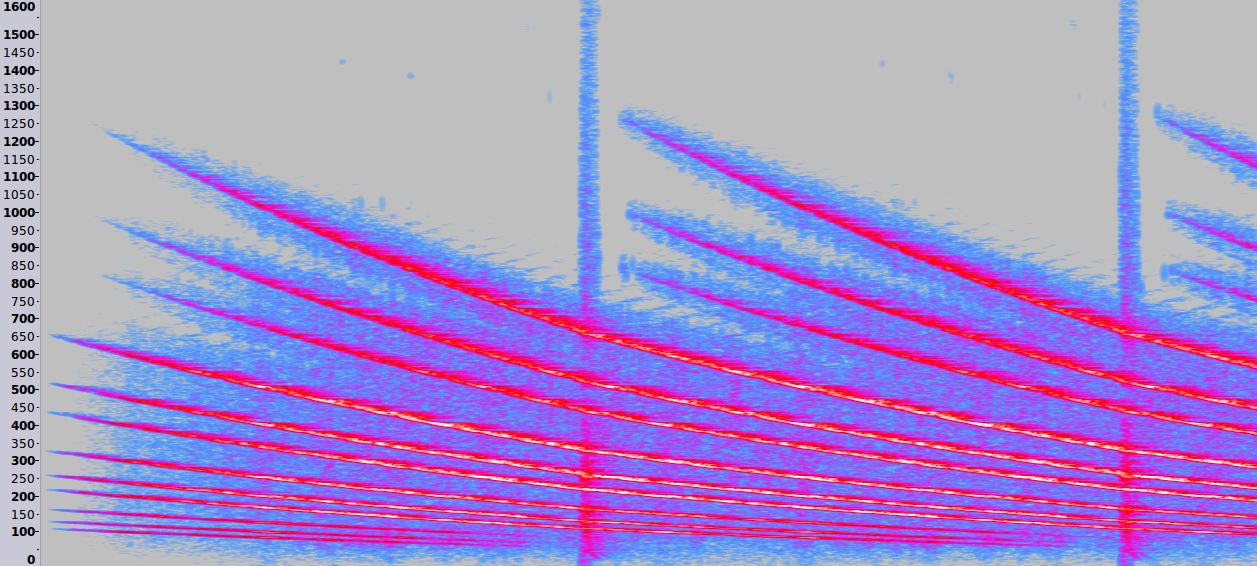
\includegraphics[width=\textwidth]{images/glissando-spectrum.png}
\end{frame}

\begin{frame}
  \frametitle{Een oneindig versnellende beat}
\end{frame}

\begin{frame}
  \frametitle{Paradox van Risset}
\end{frame}
\end{document}

